\documentclass[a4paper]{article}
\usepackage[utf8]{inputenc}
\usepackage[spanish, es-tabla, es-noshorthands]{babel}
\usepackage[table,xcdraw]{xcolor}
\usepackage[a4paper, footnotesep = 1cm, width=20cm, top=2.5cm, height=25cm, textwidth=18cm, textheight=25cm]{geometry}
%\geometry{showframe}

\usepackage{tikz}
\usepackage{amsmath}
\usepackage{amsfonts}
\usepackage{amssymb}
\usepackage{float}
\usepackage{graphicx}
\usepackage{caption}
\usepackage{subcaption}
\usepackage{multicol}
\usepackage{multirow}
\setlength{\doublerulesep}{\arrayrulewidth}
\usepackage{booktabs}

\usepackage{hyperref}
\hypersetup{
    colorlinks=true,
    linkcolor=blue,
    filecolor=magenta,      
    urlcolor=blue,
    citecolor=blue,    
}

\newcommand{\quotes}[1]{``#1''}
\usepackage{array}
\newcolumntype{C}[1]{>{\centering\let\newline\\\arraybackslash\hspace{0pt}}m{#1}}
\usepackage[american]{circuitikz}
\usetikzlibrary{calc}
\usepackage{fancyhdr}
\usepackage{units} 

\graphicspath{{../Ejercicio-1/}{../Ejercicio-2/}{../Ejercicio-3/}{../Ejercicio-4/}}

\pagestyle{fancy}
\fancyhf{}
\lhead{22.01 Teoría de Circuitos}
\rhead{Mechoulam, Lambertucci, Rodriguez Turco, Londero, Galdeman}
\rfoot{\centering \thepage}

\begin{document}

%%%%%%%%%%%%%%%%%%%%%%%%%
%		Caratula		%
%%%%%%%%%%%%%%%%%%%%%%%%%

\begin{titlepage}
\newcommand{\HRule}{\rule{\linewidth}{0.5mm}}
\center
\mbox{\textsc{\LARGE \bfseries {Instituto Tecnológico de Buenos Aires}}}\\[1.5cm]
\textsc{\Large 22.01 Teoría de Circuitos}\\[0.5cm]


\HRule \\[0.6cm]
{ \Huge \bfseries Trabajo práctico N$^{\circ}$5}\\[0.4cm] 
\HRule \\[1.5cm]


{\large

\emph{Grupo 3}\\
\vspace{3px}

\begin{tabular}{lr} 	
\textsc{Mechoulam}, Alan  &  58438\\
\textsc{Lambertucci}, Guido Enrique  & 58009 \\
\textsc{Rodriguez Turco}, Martín Sebastian  & 56629 \\
\textsc{Londero Bonaparte}, Tomás Guillermo  & 58150 \\
\textsc{Galdeman}, Agustín & 59827\\
\end{tabular}

\vspace{20px}

\emph{Profesores}\\
Jacoby, Daniel Andrés\\
Belaustegui Goitia, Carlos\\
Iribarren, Rodrigo Iñaki\\
\vspace{3px}
%\textsc{} \\	

\vspace{100px}

\begin{tabular}{ll}

Presentado: & */*/19\\

\end{tabular}

}

\vfill

\end{titlepage}


%%%%%%%%%%%%%%%%%%%%%
%		Indice		%
%%%%%%%%%%%%%%%%%%%%%

\tableofcontents
\newpage

%%%%%%%%%%%%%%%%%%%%%
%		Informe		%
%%%%%%%%%%%%%%%%%%%%%
\begin{table}[]
\centering
\begin{tabular}{|c|c|}
\hline
\textbf{$f_p^-$} & 11.712 kHz   \\ \hline
\textbf{$f_a^-$} & 13.802kHz    \\ \hline
\textbf{$f_a^+$} & 16.301kHz    \\ \hline
\textbf{$f_p^+$} & 19.211kHz    \\ \hline
\textbf{$A_a$}   & 45dB         \\ \hline
\textbf{$A_p$}   & 1dB          \\ \hline
\textbf{k}       & $\frac{1}{3}$ \\ \hline
\end{tabular}
\caption{Plantilla del filtro realizado.}
\end{table}

\begin{figure}[H]
\centering
	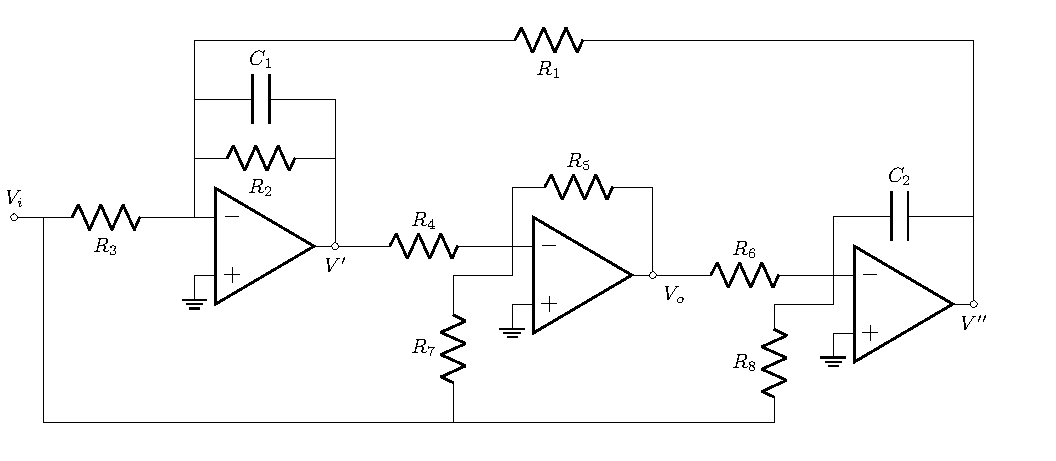
\includegraphics[width=0.9\textwidth]{Imagenes/FT.pdf}
	\caption{Circuito de la celda Universal Fleischer-Tow.}
\label{fig:circft}
\end{figure}

Elección de componentes:
\begin{table}[H]
\centering
\begin{tabular}{ccc}
\hline
\multicolumn{1}{c}{Componente} & \multicolumn{1}{c}{Valor} & Composición \\ \hline
$R_1$                           & 33.68K                     & 680+33K     \\
$R_2$                           & 334.28K                    & 3.9K+330K   \\
$R_3$                           & 47K                        & 47K         \\
$R_4$                           & 334.28K                    & 3.9K+330K   \\
$R_5$                           & 47K                        & 47K         \\
$R_6$                           & 49.7K                        & 2.7k+47k         \\
$R_7$                           & 47K                        & 47K         \\
$R_8$                           & 50K                        & 47K+3k         \\
$C_1$                           & 95P                        & 68p//27p     \\
$C_2$                           & 95P                        & 68p //27p    \\
\hline
\end{tabular}
\caption{Componentes seleccionados de la primer etapa.}
\end{table}

\begin{table}[H]
\centering
\begin{tabular}{ccc}
\hline
\multicolumn{1}{c}{Componente} & \multicolumn{1}{c}{Valor} & Composición  \\ \hline
$R_1$                           & 27.03                      & 27+27K      \\
$R_2$                           & 371.57k                    & 680k // 820k \\
$R_3$                           & 47k                        & 47k          \\
$R_4$                           & 371.57k                    & 680k //820k   \\
$R_5$                           & 52.5k                      & 56k//820k    \\
$R_6$                           & 49.77k                     & 2.7k+47k     \\
$R_7$                           & 47k                        & 47k          \\
$R_8$                           & 47.5k                        & 47k+500          \\
$C_1$                           & 100p                       & 100p         \\
$C_2$  \\
\hline
\end{tabular}
\caption{Componentes seleccionados de la segunda etapa.}
\end{table}

\begin{table}[H]
\centering
\begin{tabular}{ccc}
\hline
\multicolumn{1}{c}{Componente} & \multicolumn{1}{c}{Valor} & Composición \\ \hline
$R_1$                           & 27.13                      & 120+27k     \\
$R_2$                           & 465.31k                    & 680k//1.5M  \\
$R_3$                           & 47k                        & 47k         \\
$R_4$                           & 465.31k                    & 680k//1.5M  \\
$R_5$                           & 42.08k                     & 15k+27k     \\
$R_6$                           & 49.77k                     & 2.7k+47k    \\
$R_7$                           & 47k                        & 47k         \\
$R_8$                           & 48k                        & 47k+1k         \\
$C_1$                           & 100p                       & 100p        \\
$C_2$                           & 100p                       & 100p        \\
\hline
\end{tabular}
\caption{Componentes seleccionados de la tercer etapa.}
\end{table}

\begin{table}[H]
\centering
\begin{tabular}{ccc}
\hline
\multicolumn{1}{c}{Componente} & \multicolumn{1}{c}{Valor} & Composición \\ \hline
$R_1$                           & 10.29k                     & 4.7k+5.6k   \\
$R_2$                           & 1.32M                      & 120k+1.2M   \\
$R_3$                           & 47k                        & 47k         \\
$R_4$                           & 1.32M                      & 120k+1.2M   \\
$R_5$                           & 39.44k                     & 470+39k     \\
$R_6$                           & 49.77K                     & 2.7k+47k    \\
$R_7$                           & 47k                        & 47k         \\
$R_8$                           & 48k                        & 47k+1k         \\
$C_1$                           & 92p                        & 10p // 82p  \\
$C_2$                           & 92p                        & 10p // 82p  \\
\hline
\end{tabular}
\caption{Componentes seleccionados de la cuarta etapa.}
\end{table}

\begin{table}[H]
\centering
\begin{tabular}{ccc}
\hline
\multicolumn{1}{c}{Componente} & \multicolumn{1}{c}{Valor} & Composición \\ \hline
$R_1$                           & 10.19k                     & 12k//68k    \\
$R_2$                           & 918.2k                     & 100k+820k   \\
$R_3$                           & 47k                        & 47k         \\
$R_4$                           & 918.2k                     & 100k+820k   \\
$R_5$                           & 56k                        & 56k         \\
$R_6$                           & 49.77k                     & 2.7k+47k    \\
$R_7$                           & 45k                        & 43k+2k         \\
$R_8$                           & 55k                        & 12k+43k         \\
$C_1$                           & 88p                      & 82p//5.6p    \\
$C_2$                           & 88p                      & 82p//5.6p   \\
\hline
\end{tabular}
\caption{Componentes seleccionados de la quinta etapa.}
\end{table}

\begin{table}[H]
\centering
\begin{tabular}{ccc}
\hline
\multicolumn{1}{c}{Componente} & \multicolumn{1}{c}{Valor} & Composición \\ \hline
$R_1$                           & 27.13                      & 120+27k     \\
$R_2$                           & 465.31k                    & 680k//1.5M  \\
$R_3$                           & 47k                        & 47k         \\
$R_4$                           & 465.31k                    & 680k//1.5M  \\
$R_5$                           & 42.08k                     & 15k+27k     \\
$R_6$                           & 49.77k                     & 2.7k+47k    \\
$R_7$                           & 46k                        & 43k+3k         \\
$R_8$                           & 53k                        & 51k+2k         \\
$C_1$                           & 70p                       & 68p        \\
$C_2$                           & 70p                       & 68p  \\
\hline
\end{tabular}
\caption{Componentes seleccionados de la sexta etapa.}
\end{table}
\end{document}